\documentclass[10pt,handout]{beamer}

\usetheme{metropolis}
\usepackage{appendixnumberbeamer,amsmath}
\usepackage[ruled,vlined]{algorithm2e}
\usepackage{booktabs}
\usepackage[scale=2]{ccicons}

\usepackage{pgfplots}
\usepgfplotslibrary{dateplot}
\usepackage{tikz}
\usetikzlibrary{positioning}

\usepackage{xspace}
\newcommand{\themename}{\textbf{\textsc{metropolis}}\xspace}
\DeclareMathOperator{\order}{Order}

\usepackage{libertine}
\usepackage[libertine]{newtxmath}
\usepackage{mathrsfs}
\usepackage{silence}
\WarningFilter{latexfont}{Size substitutions}
\WarningFilter{latexfont}{Font shape}
\title{Deterministic List Decoding of Reed Solomon Codes}
% \subtitle{Derandomizing Sudan and Guruswami-Sudan Algorithm}
\date{\today}
\author{Soham Chatterjee}
% \institute{ISI Seminar}
\renewcommand{\thealgocf}{}
% \titlegraphic{\hfill
\includegraphics[height=1.5cm]{logo.pdf}}
\metroset{block=fill}
\pagestyle{empty}
\input{../../letterfonts.tex}
\DeclareMathOperator{\poly}{poly}
\usepackage[backend=bibtex, style=alphabetic, maxnames=3]{biblatex}
\addbibresource{deterministicgs.bib}
\begin{document}
\maketitle

% \begin{frame}{Table of contents}
% 	\setbeamertemplate{section in toc}[sections numbered]
% 	\tableofcontents[hideallsubsections]
% \end{frame}

\section{Introduction}
\begin{frame}{What is Coding Theory?}
	Suppose you want to send a message to your friend over a \textcolor{blue}{noisy channel} --- some symbols can change arbitrarily.
	\vspace{0.4em}
	\begin{center}
		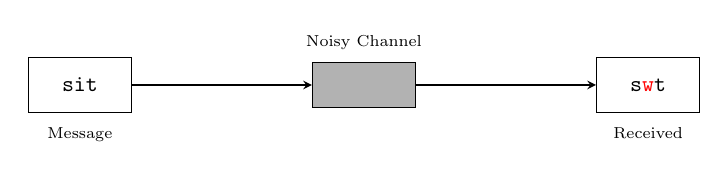
\begin{tikzpicture}[>=stealth, scale=0.82, transform shape]
			% --- Row 1: raw channel, no encoding ---
			\node[draw, rectangle, minimum width=1.6cm, minimum height=0.85cm, align=center]
			(m) at (0, 0) {\texttt{sit}};
			\node[font=\scriptsize, below=3pt of m] {Message};

			\node[draw, rectangle, fill=gray!60, minimum width=1.6cm, minimum height=0.7cm]
			(ch1) at (4.4, 0) {};
			\node[font=\scriptsize, above=2pt of ch1] {Noisy Channel};

			\node[draw, rectangle, minimum width=1.6cm, minimum height=0.85cm, align=center]
			(v) at (8.8, 0) {\texttt{s\textcolor{red}{w}t}};
			\node[font=\scriptsize, below=3pt of v] {Received};

			\draw[->] (m.east) -- (ch1.west);
			\draw[->] (ch1.east) -- (v.west);
		\end{tikzpicture}
	\end{center}
	You sent \texttt{sit}, but received \texttt{s\textcolor{red}{w}t} --- the symbol \texttt{i} got corrupted to \texttt{\textcolor{red}{w}}. What was the original message?

	\onslide<2->{\vspace{0.3em}\textbf{Solution:} \textcolor{blue}{Encode} $\mathbf{m}$ before sending; \textcolor{blue}{decode} $\mathbf{v}$ after receiving.}
	\begin{center}
		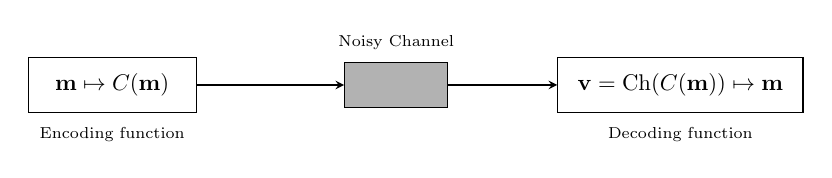
\begin{tikzpicture}[>=stealth, scale=0.82, transform shape]
			\onslide<2->{
			\node[draw, rectangle, minimum width=2.6cm, minimum height=0.85cm, align=center]
			(enc) at (0, -2.4) {$\mathbf{m} \mapsto C(\mathbf{m})$};
			\node[font=\scriptsize, below=3pt of enc] {Encoding function};

			\node[draw, rectangle, fill=gray!60, minimum width=1.6cm, minimum height=0.7cm]
			(ch2) at (4.4, -2.4) {};
			\node[font=\scriptsize, above=2pt of ch2] {Noisy Channel};

			\node[draw, rectangle, minimum width=3.8cm, minimum height=0.85cm, align=center]
			(dec) at (8.8, -2.4) {$\mathbf{v}=\mathrm{Ch}(C(\mathbf{m}))\mapsto\mathbf{m}$};
				\node[font=\scriptsize, below=3pt of dec] {Decoding function};

				\draw[->] (enc.east) -- (ch2.west);
				\draw[->] (ch2.east) -- (dec.west);
			}
		\end{tikzpicture}
	\end{center}
	\vspace{0.1em}

\end{frame}

\begin{frame}{A Simple Idea: Repetition Code}
	\textbf{Idea:} Send the same message $3$ times: $\texttt{sit} \to \texttt{sitsitsit}$.\pause
	\vspace{0.5em}

	\begin{block}{Decoding by majority}
		For each coordinate, take the \textcolor{blue}{majority} over the three copies. A single symbol-flip anywhere is corrected.
	\end{block}\pause
	\vfill

	\textbf{Problem:} The codeword is $3\times$ as long as the message. To handle more errors we'd need even more copies. This is \textcolor{blue}{too wasteful}! \pause

\end{frame}

\begin{frame}{Solution}
	We want a \textcolor{blue}{smarter encoding} that corrects errors without a large blowup in length.

	\vspace{0.7em}
	With this in place, let us set up some notation\ldots

	\vfill
	\begin{block}{Key Assumption}
		The number of errors is \textcolor{blue}{bounded} --- the channel cannot corrupt the entire word.
	\end{block}

\end{frame}

\begin{frame}{Introduction to Coding Theory}
	We now introduce a few terminologies used in coding theory.
	\vspace{0.5em}\pause

	Let $\textcolor{blue}{\mcM}$ be the \textbf{message space} and $\textcolor{blue}{\Sg}$ a finite \textbf{alphabet}. A code is a family of maps, one for each length of codeword:\pause
	\begin{itemize}
		\item \textbf{Encoding:} $\textcolor{blue}{\mathrm{Enc}_n : [|\mcM|] \to \Sg^n}$\pause
		\item \textbf{Decoding:} $\textcolor{blue}{\mathrm{Dec}_n : \Sg^n \to [|\mcM|]}$
	\end{itemize}\pause

	The image $\textcolor{blue}{\mcC = \mathrm{Enc}_n([|\mcM|]) \subseteq \Sg^n}$ is the \textbf{code}; its elements are \textbf{codewords}.\pause

	\begin{itemize}
		\item \textbf{Blocklength:} $\textcolor{blue}{n}$\pause
		\item \textbf{Dimension:} $\textcolor{blue}{k = \log|\mcC|}$\pause
		\item \textbf{Rate:} $\textcolor{blue}{R(\mcC) = \dfrac{k}{n\log|\Sg|}}$
	\end{itemize}
\end{frame}

\begin{frame}{Introduction to Coding Theory}
	The \textbf{Hamming distance} between $\textcolor{blue}{u, v \in \Sg^n}$ is the number of coordinates where they differ:
	$$\textcolor{blue}{\Dl(u,v) \;=\; \bigl|\{\,i : u_i \neq v_i\,\}\bigr|}$$\pause

	\begin{itemize}
		\item \textbf{Distance of code:} $\textcolor{blue}{\Dl(\mcC)=\min\limits_{c_1\neq c_2\in\mcC}\Dl(c_1,c_2)}$\pause
		\item \textbf{Relative distance:} $\textcolor{blue}{\dl(\mcC)=\dfrac{\Dl(\mcC)}{n}}$
	\end{itemize}\pause

	\vspace{0.4em}
	Intuitively: a large distance means codewords are far apart, making it easier to recover from errors.\pause

	\vspace{0.3em}
	The set $\textcolor{blue}{\{u\in\Sg^n : \Dl(u,v)\leq r\}}$ is a \textbf{Hamming ball} of \textbf{radius} $\textcolor{blue}{r}$ around $\textcolor{blue}{v}$. We often speak of decoding \emph{radius} rather than distance.
\end{frame}

\begin{frame}{Introduction to Coding Theory}
	\textbf{Goal:} Construct codes such that
	\begin{itemize}
		\item Codewords to be ``far apart'' from each other $\implies$ \textcolor{blue}{High Distance}\pause
		\item Redundancy to be low $\implies$ \textcolor{blue}{High Rate}
	\end{itemize}\pause

	\begin{block}{Relation between Rate and Distance}
		For any code $\textcolor{blue}{\mcC}$ $$\textcolor{blue}{k\leq n-d+1}$$
		Asymptotically $\textcolor{blue}{R+\dl\leq 1}$ as $\textcolor{blue}{n}$ becomes very large.
	\end{block}\pause

	Codes achieving this bound are called \textbf{Maximum Distance Separable (MDS)} codes.
	\begin{itemize}
		\item Reed Solomon Codes are MDS codes.
	\end{itemize}
\end{frame}

\begin{frame}{Unique Decoding}
	\begin{center}
		\begin{minipage}{0.55\textwidth}

			Let $\textcolor{blue}{\Dl(\mcC)=d}$. For any $\textcolor{blue}{v\in\Sg^n}$ there is at most one codeword $\textcolor{blue}{c\in\mcC}$ such that $\textcolor{blue}{\Dl(v,c)\leq  (d-1)/2}$.
		\end{minipage}
		\begin{minipage}{0.42\textwidth}
			\centering
			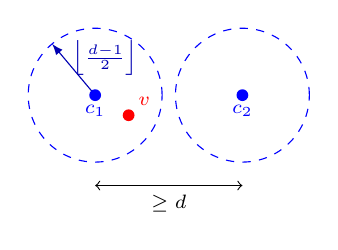
\begin{tikzpicture}[scale=0.85]
				% Disjoint Hamming balls around c_1 and c_2
				\draw[blue, dashed] (-1.1, 0) circle (1.0cm);
				\draw[blue, dashed] (1.1, 0) circle (1.0cm);

				% Radius label on c_1's ball
				\draw[-latex, blue!70!black] (-1.1,0) -- node[midway,font=\scriptsize, above,yshift=-2mm, xshift=4mm]{$\left\lfloor\tfrac{d-1}{2}\right\rfloor$} ++(130:1.0cm);

				% Codewords
				\fill[blue]           (-1.1, 0) circle (2.5pt)
				node[below, blue, font=\scriptsize] {$c_1$};
				\fill[blue] (1.1, 0) circle (2.5pt)
				node[below, blue, font=\scriptsize] {$c_2$};

				% Received word inside c_1's ball only
				\fill[red] (-0.6, -0.3) circle (2.5pt)
				node[above right, red, font=\scriptsize] {$v$};

				% Distance >= d between the two codewords
				\draw[<->, black, thin] (-1.1,-1.35) -- (1.1,-1.35)
				node[midway, below, black, font=\scriptsize] {$\geq d$};
			\end{tikzpicture}
		\end{minipage}
	\end{center}\pause

	\textbf{Unique Decoding Problem:} Given a received word $\textcolor{blue}{v\in\Sg^n}$, find the unique codeword $\textcolor{blue}{c\in\mcC}$ such that $\textcolor{blue}{\Dl(v,c)< d/2}$ if it exists.\pause
	\begin{itemize}
		\item If we go more than $\textcolor{blue}{d/2}$ distance, multiple codewords may lie in the radius of hamming ball.
	\end{itemize}
\end{frame}

\begin{frame}{List Decoding}
	\begin{center}
		\begin{minipage}{0.54\textwidth}
			\begin{definition}[$\textcolor{blue}{(\rho,L)}$-List Decodable]
				$\textcolor{blue}{\mcC}$ is $\textcolor{blue}{(\rho,L)}$-list decodable if for every $\textcolor{blue}{v\in\Sg^n}$,
				$$\textcolor{blue}{|\{c\in\mcC\mid \Dl(c,v)\leq \rho n\}|\leq L}$$
			\end{definition}
		\end{minipage}
		\hfill
		\begin{minipage}{0.42\textwidth}
			\centering
			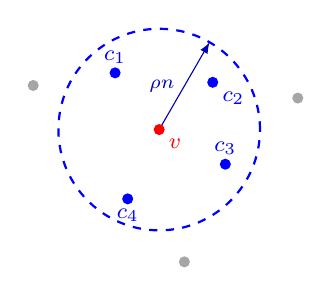
\begin{tikzpicture}[scale=0.8]
				% Hamming ball of radius rho*n around v
				\draw[blue, thick, dashed] (0,0) circle (1.6cm);

				% Radius label
				\draw[-latex, blue!70!black] (0,0) -- ++(60:1.6cm) node[blue!70!black, font=\scriptsize, midway, left]{$\rho n$};
				% Received word v at center
				\fill[red] (0,0) circle (2.5pt)
				node[below right, red, font=\footnotesize] {$v$};

				% Codewords inside the ball
				\fill[blue] (-0.7, 0.9) circle (2.5pt)
				node[above, blue, font=\footnotesize] {$c_1$};
				\fill[blue] (0.85, 0.75) circle (2.5pt)
				node[below right, blue, font=\footnotesize] {$c_2$};
				\fill[blue] (1.05, -0.55) circle (2.5pt)
				node[above, blue, font=\footnotesize] {$c_3$};
				\fill[blue] (-0.5, -1.1) circle (2.5pt)
				node[below, blue, font=\footnotesize] {$c_4$};

				% Codewords outside (grayed out)
				\fill[gray!70] (2.2, 0.5) circle (2.5pt);
				\fill[gray!70] (-2.0, 0.7) circle (2.5pt);
				\fill[gray!70] (0.4, -2.1) circle (2.5pt);
			\end{tikzpicture}
		\end{minipage}
	\end{center}
	\vspace{0.3em}

	We write $\textcolor{blue}{L(v,\rho)=\{c\in\mcC\mid \Dl(c,v)\leq \rho n\}}$.

	\vspace{0.5em}
	Unlike unique decoding, \textcolor{blue}{multiple codewords} may lie inside the ball --- we output the entire list $L(v)$.
\end{frame}

\begin{frame}{List Decoding}
	\textbf{List Decoding Problem:} Given a received word $\textcolor{blue}{v\in \Sg^n}$, compute $\textcolor{blue}{L(v,\rho)}$.\pause
	\begin{itemize}
		\item \textbf{Combinatorial:} Prove $\textcolor{blue}{|L(v,\rho)|=\poly(n)}$\pause
		\item \textbf{Algorithmic:} Find all codewords in $\textcolor{blue}{L(v,\rho)}$ in $\textcolor{blue}{\poly(n)}$ time.
	\end{itemize}\pause
	\vspace{0.5em}

	\begin{theorem}[Johnson Bound]
		For a code $\textcolor{blue}{\mcC}$ with rate $\textcolor{blue}{R}$, the list size is polynomial in $\textcolor{blue}{n}$ for $\textcolor{blue}{\rho\leq 1-\sqrt{R}}$.
	\end{theorem}\pause

	\vspace{0.6em}
	\textbf{Convention:} We use \textcolor{blue}{agreement} $t = 1-\rho$ in place of error fraction $\rho$.
\end{frame}

\begin{frame}{Why Polynomial-Based Codes?}
	We want codes with \textcolor{blue}{high rate} and \textcolor{blue}{large distance}. A natural question: what mathematical structure should we build on?\pause

	\vspace{0.5em}
	\textbf{Answer:} Polynomials are nice to use.
	\vspace{0.4em}

	\begin{itemize}
		\item  The algebra of polynomials is classical and rich.\pause
		\item  Polynomial arithmetic can all be done very efficiently. All the basic operations in near linear time.\pause
		\item Connections to algebra, number theory, and algebraic geometry give powerful tools for both encoding and decoding.
	\end{itemize}
	\vspace{1em}

	\textbf{Examples:} Reed-Solomon Codes, Reed-M\"{u}ller Codes, BCH Codes, Multiplicity Codes\ldots
\end{frame}

\section{Reed Solomon Codes (RS)}
\begin{frame}{Construction}
	Fix a finite field $\textcolor{blue}{\bbF_q}$ and distinct evaluation points $\textcolor{blue}{S=\{\alpha_1,\dots,\alpha_n\}\subseteq \bbF_q}$.\pause

	\vspace{0.3em}
	$\textcolor{blue}{RS[n,k]_q}$: each message $\textcolor{blue}{m}$ is identified with a polynomial $\textcolor{blue}{f_m\in\bbF_q[X]}$ of degree $\textcolor{blue}{<k}$, and encoded by evaluating at all points of $S$:
	$$\textcolor{blue}{\mathrm{Enc}(m) = \bigl(f_m(\alpha_1),\, f_m(\alpha_2),\, \dots,\, f_m(\alpha_n)\bigr)}$$\pause

	\textbf{Rate}: $\textcolor{blue}{k/n}$.\pause

	\vspace{0.4em}
	Codewords form a \textcolor{blue}{vector space}, so $\Dl(\mcC) = $ min nonzero positions of any nonzero codeword $= $ min nonzero evaluations of a nonzero $\deg < k$ polynomial.\pause

	\textbf{Distance:} $\textcolor{blue}{d = n - k + 1}$

	This meets the Singleton bound $d \leq n-k+1$, making RS codes \textbf{MDS}.
\end{frame}

\begin{frame}{Reed Solomon Decoding History}
	\textbf{Goal:} Decode in $\textcolor{blue}{\poly(n,\log q)}$ time or \textcolor{blue}{$\poly(n)$} field operations.
	\vspace{0.6em}\pause

	Unique Decoding Radius: \textcolor{blue}{$>(n+k-1)/2$}

	Johnson radius for \textcolor{blue}{$RS[n,k]_q$}: agreement \textcolor{blue}{$> \sqrt{n(k-1)}$}.\pause

	\textbf{Good news:} all three settings above admit \textcolor{blue}{$\poly(n)$} algorithms.\pause

	\begin{tabular*}{\textwidth}{@{\extracolsep{\fill}} l c l @{}}
		\textbf{Algorithm} & \textbf{Agreement} & \uncover<5->{\textbf{Type}} \\[4pt]\hline\\[-6pt]
		Berlekamp--Welch     & \textcolor{blue}{$> (n+k-1)/2$}      & \uncover<5->{deterministic} \\[4pt]
		Sudan '97            & \textcolor{blue}{$> \sqrt{2n(k-1)}$} & \uncover<5->{randomized}    \\[4pt]
		Guruswami--Sudan '99 & \textcolor{blue}{$> \sqrt{n(k-1)}$}  & \uncover<5->{randomized}    \\[4pt]
	\end{tabular*}

	\vspace{0.3em}
	\onslide<6->{The \textcolor{blue}{deterministic} variant of GS runs in \textcolor{blue}{$\poly(n)$} but with \textcolor{blue}{polynomial dependence on the field characteristic}.}
\end{frame}

\begin{frame}{Framework of Sudan and Guruswami-Sudan}
	Let $\textcolor{blue}{w = \{(\alpha_j, \beta_j)\}_{j\in[n]}}$ be the received word. Both algorithms share the same two-step structure:\pause

	\vspace{0.5em}
	\textbf{Step 1: Interpolation.}
	Find a nonzero bivariate polynomial $\textcolor{blue}{Q(X,Y) \in \bbF_q[X,Y]}$ vanishing at every received point $\textcolor{blue}{(\alpha_j, \beta_j)}$ with some multiplicity, chosen 
	
	So that every close codeword $\textcolor{blue}{f}$ satisfies $\textcolor{blue}{(Y - f(X)) \mid Q(X,Y)}$.\pause

	\vspace{0.3em}
	\textit{Sudan uses multiplicity $\textcolor{blue}{1}$; Guruswami--Sudan uses higher multiplicity $\textcolor{blue}{m>1}$ to push the radius further.}\pause

	\vspace{0.5em}
	\textbf{Step 2: Factorization.}
	Completely factor $\textcolor{blue}{Q(X,Y)}$ over $\textcolor{blue}{\bbF_q}$ and collect all factors of the form $\textcolor{blue}{Y - f(X)}$
\end{frame}

\begin{frame}{Factorization Barrier}
	
	
	The \textcolor{blue}{interpolation step is already deterministic}. The bottleneck is the \textcolor{blue}{factorization step}.\pause
	
	Both Sudan and Guruswami–Sudan algorithms rely heavily on the factorization of bivariate polynomials over finite fields
	\vspace{0.4em}

	In fact, the difficulty already appears in the \textcolor{blue}{univariate} case: factoring a degree-$\textcolor{blue}{d}$ polynomial over $\textcolor{blue}{\bbF_q}$ deterministically in $\textcolor{blue}{\poly(d, \log q)}$ time is \textbf{open}.\pause

	\begin{itemize}
		\item \textbf{Berlekamp}, \textbf{Cantor--Zassenhaus}: randomized $\textcolor{blue}{\poly(d,\log q)}$ algorithms for univariate factoring over $\textcolor{blue}{\bbF_q}$.\pause
		\item Deterministic variants run in time \textbf{polynomial in the field characteristic} . Too slow when the characteristic is large (super polynomial)
	\end{itemize}\pause

	\vspace{0.3em}
	\textbf{State of Art:} No known truly deterministic $\textcolor{blue}{\poly(n,\log q)}$ factorization or RS-list decoding algorithm existed.
\end{frame}

\begin{frame}{Our Result}
	We give the \textcolor{blue}{first truly deterministic} polynomial-time list decoding algorithm for Reed--Solomon codes, matching the running time of the Sudan and Guruswami--Sudan algorithms.

	\vspace{0.5em}

	\textbf{Key contribution:} a deterministic algorithm for the factorization step --- finding all factors of $\textcolor{blue}{Q(X,Y)}$ of the form $\textcolor{blue}{Y-f(X)}$ in $\textcolor{blue}{\poly(n)}$ field operations, with no dependence on the field characteristic.
	\vfill

	\begin{theorem}[\cite{ChatterjeeHK2025}]
		There is a deterministic algorithm that, for every finite field $\bbF$ and parameters $n > k \in \bbN$, runs in time $\poly(n, \log |\bbF|)$ and list decodes $RS[n,k]_{\bbF}$ from agreement greater than $\sqrt{(k-1)n}$.
	\end{theorem}

	\vspace{0.4em}
\end{frame}

\section{Derandomization of Sudan}
\begin{frame}{Newton Iteration}

	Let $\textcolor{blue}{P(X,Y)\in\bbF_q[X,Y]}$ and $\textcolor{blue}{f(X)\in\bbF_q[X]}$ such that
	\begin{itemize}
		\item $\textcolor{blue}{P(X,f(X))\equiv 0}$ \pause
		\item $\textcolor{blue}{\alpha\in\bbF_q}$ such that $\textcolor{blue}{\frac{\partial}{\partial Y}P(\alpha, f(\alpha))\neq 0}$.\pause
		\item $\textcolor{blue}{Y_t=f(X)\mod X^t}$ for all $\textcolor{blue}{t\in\bbN}$
	\end{itemize}\pause

	Newton Iteration gives an efficient way to compute $\textcolor{blue}{Y_{t+1}}$ from $\textcolor{blue}{Y_t}$ as follows:\pause
	$$\textcolor{blue}{Y_{t+1}=Y_t-\frac{P(X,Y_t)}{\partial_YP(X,Y_t)}}$$
\end{frame}
\begin{frame}{Sudan Derandomization}
	Let $\textcolor{blue}{f}$ is in the list. And let $\textcolor{blue}{j\in[n]}$ such that $\textcolor{blue}{f(\alpha_j)=\beta_j}$. Suppose $\textcolor{blue}{Q}$ is the polynomial from interpolation step.\pause
	\vfill

	If $\textcolor{blue}{\partial_Y Q(\alpha_j,f(\alpha_j))\neq 0}$:
	Then Newton Iteration from $\textcolor{blue}{Y_0}$ till $\textcolor{blue}{Y_k}$ gives $\textcolor{blue}{f}$. \pause\vfill

	Else $\textcolor{blue}{\partial_Y Q(\alpha_j,f(\alpha_j))=0}$ for all $\textcolor{blue}{j}$ in agreement.\pause \vfill

	\textbf{Observe:} $\textcolor{blue}{\partial_Y(Q(X,f(X)))}$ has more than $\textcolor{blue}{\sqrt{2n(k-1)}}$ roots but degree at most $\textcolor{blue}{\sqrt{2n(k-1)}}$.
	Implying $\textcolor{blue}{\partial_Y(Q(X,f(X)))\equiv 0}$\pause

	So recurse on $\textcolor{blue}{\partial_Y(Q(X,f(X)))}$.
\end{frame}
\begin{frame}{Sudan Derandomization}
	\textbf{Algorithm:}
	\begin{enumerate}
		\item Check for each $\textcolor{blue}{j\in[n]}$ if $\textcolor{blue}{\partial_Y Q(\alpha_j,\beta_j)\neq0}$. If yes, do Newton Iteration from there.\pause
		\item Else compute $\textcolor{blue}{\partial_Y(Q(X,Y))}$ and continue from step 1 with $\textcolor{blue}{\partial_YQ(X,Y)}$ instead of $\textcolor{blue}{Q}$.
	\end{enumerate} \pause\vfill

	\begin{theorem}
		There is a deterministic algorithm that, for every finite field $\textcolor{blue}{\bbF}$ and parameters $\textcolor{blue}{n,k\in\bbN}$ runs in time $\textcolor{blue}{\poly(n,\log|\bbF|)}$ list decodes Reed Solomon code $\textcolor{blue}{RS[n,k]}$ from agreement more than $\textcolor{blue}{\sqrt{2n(k-1)}}$.
	\end{theorem}
\end{frame}
\section{Derandomization of Guruswami-Sudan}

\begin{frame}{Local Splitting}
	Let $\textcolor{blue}{P(X,Y)\in \bbF_q[X,Y]}$ with no-pure $\textcolor{blue}{X}$-factors. Let $\textcolor{blue}{(\alpha,\beta)\in\bbF_q^2}$ any point.\pause

	Suppose we are given the factorization $\textcolor{blue}{P=\prod_{i=1}^s P_i}$ into irreducibles (with multiplicity)\pause

	Eg: $\textcolor{blue}{P(X,Y)=(Y^2+X)(Y^2+X+1)^2}$ then
	$$\textcolor{blue}{P_1=Y^2+X, \quad P_2=Y^2+X+1, \quad P_3=Y^2+X+1}$$\pause

	We partition $\textcolor{blue}{[s]}$ into four sets which defines four types of factors at $\textcolor{blue}{(\alpha,\beta)}$:
	$$\textcolor{blue}{A(\alpha,\beta),\quad B(\alpha,\beta),\quad C(\alpha,\beta),\quad D(\alpha,\beta)}$$
\end{frame}
\begin{frame}{Local Splitting}
	Let $P(X,Y)=(Y^2+X+1)(Y^2+X)(Y^2+X^2+Y)(XY+1)$ and  $(\alpha,\beta)=(0,0)$\pause
	\begin{itemize}
		\item $A(\alpha,\beta)= \{i\in[s]\mid P_i(\alpha,\beta)\neq 0, \deg(P_i(\alpha,Y))\geq 1\}$\pause

		      So $Y^2+X+1\in A(0,0)$\pause
		\item $		B(\alpha,\beta) = \{i\in[s]\mid P_i(\alpha,Y)=\gm(Y-\beta)^m,m\geq 1,\gm\neq 0\}$\pause

		      So $Y^2+X\in B(0,0)$\pause
		\item $C(\alpha,\beta) =\{i\in[s]\mid P_i(\alpha,Y)=(Y-\beta)^m\hat{P}_i(Y),m\geq 1, \hat{P}_i(\beta)\neq 0, \deg \hat{P}_i\geq 1\}$\pause

		      So $Y^2+X^2+Y\in C(0,0)$\pause
		\item $D(\alpha,\beta) =\{i\in[s]\mid P_i(\alpha,\beta)\neq 0, \deg(P_i(\alpha,Y))=0\}$\pause

		      So $XY+1\in D(0,0)$
	\end{itemize}\pause

	I will use $A,B,C,D$ to denote these. Define $P_A=\prod_{i\in A} P_i$ and similarly $P_B,P_C,P_D$.\pause

	\textbf{Observe: }If $P$ is monic in $Y$ then $D$ is empty.
\end{frame}

\begin{frame}{A Nice Observation}
	$\textcolor{blue}{w=\{(\alpha_j,\beta_j)\}_{j\in[n]}}$ denote the received word.

	$\textcolor{blue}{Q}$ is the polynomial from Interpolation step of Guruswami-Sudan algorithm. Let $\textcolor{blue}{f}$ is in the list.\vspace{5mm} \pause

	For any $\textcolor{blue}{j\in[n]}$:\vspace{2mm}\pause

	\hspace{1cm} If $\textcolor{blue}{f(\alpha_j)=\beta_j}$: Then $\textcolor{blue}{Y-f(X)\mid P_B}$\vspace{2mm}\pause

	\hspace{1cm} If $\textcolor{blue}{f(\alpha_j)\neq \beta_j}$: Then $\textcolor{blue}{Y-f(X)\mid P_A}$
\end{frame}
\begin{frame}{Derandomization}
	\begin{block}{Remark}
		We will assume $\textcolor{blue}{Q}$ is monic in $\textcolor{blue}{Y}$ and has no pure $\textcolor{blue}{X}$-factors.
	\end{block}\pause

	\textbf{If only we had:} An efficient $\textcolor{blue}{\poly(n,\log q)}$ time algorithm \textsc{Split} to find $\textcolor{blue}{P_A,P_B}$ from $\textcolor{blue}{P, (\alpha,\beta)}$ then:\pause

	\textbf{Algorithm:}
	\begin{enumerate}
		\item $\textcolor{blue}{S\longleftarrow \{Q\}}$\pause
		\item Choose $\textcolor{blue}{j\in[n]}$ and for all $\textcolor{blue}{g\in S}$ compute $\textcolor{blue}{(g_A,g_B)=\textsc{Split}(g,(\alpha_j,\beta_j))}$\pause
		\item Remove $\textcolor{blue}{g}$ from $\textcolor{blue}{S}$ and put $\textcolor{blue}{g_A,g_B}$ in $\textcolor{blue}{S}$.\pause
		\item Continue from step 2 till $\textcolor{blue}{S}$ stabilizes.\pause
		\item Do some interpolations to recover list
	\end{enumerate}
\end{frame}
\begin{frame}{Recover List from Stable Set}
	\textbf{Observe:} If $\textcolor{blue}{f}$ is in the list there is one factor $\textcolor{blue}{g\in S}$, $\textcolor{blue}{Y-f(X)\mid g}$. \pause

	\begin{lemma}
		For all $\textcolor{blue}{j\in[n]}$,
		$$\textcolor{blue}{g(\alpha_j,\beta_j)=0\iff f(\alpha_j)=\beta_j}$$
	\end{lemma}\pause
	So go over all $\textcolor{blue}{g\in S}$, find $\textcolor{blue}{j\in[n]}$ such that $\textcolor{blue}{g(\alpha_j,\beta_j)=0}$, do interpolation to find appropriate $\textcolor{blue}{f}$.\pause

	\boxed{\text{But stabilization can take long time !!}}\pause

	Simple potential function:
	$$\textcolor{blue}{\Phi(S)=\sum_{i=1}^{\deg_Y(Q)}(i-1)\times \#(\text{polynomials with $Y$-deg $=i$  in $S$})}$$\pause
	You will notice $\textcolor{blue}{\Phi(S)}$ decreases by at least $\textcolor{blue}{1}$ in each update of $\textcolor{blue}{S}$.
\end{frame}
\begin{frame}{Finally}
	Final Algorithm:
	\begin{enumerate}
		\item $\textcolor{blue}{S\longleftarrow \{Q\}}$
		\item Choose $\textcolor{blue}{j\in[n]}$ and for all $\textcolor{blue}{g\in S}$ compute $\textcolor{blue}{(g_A,g_B)=\textsc{Split}(g,(\alpha_j,\beta_j))}$
		\item Remove $\textcolor{blue}{g}$ from $\textcolor{blue}{S}$ and put $\textcolor{blue}{g_A,g_B}$ in $\textcolor{blue}{S}$.
		\item Continue from step 2 till $\textcolor{blue}{S}$ stabilizes.
		\item Go over all $\textcolor{blue}{g\in S}$ and do interpolation on the set $\textcolor{blue}{\{j\in[n]\mid g(\alpha_j,\beta_j)=0\}}$ and recover list
	\end{enumerate}\vfill \pause

	\begin{theorem}
		There is a deterministic algorithm that, for every finite field $\textcolor{blue}{\bbF}$ and parameters $\textcolor{blue}{n,k\in\bbN}$ runs in time $\textcolor{blue}{\poly(n,\log|\bbF|)}$ list decodes Reed Solomon code $\textcolor{blue}{RS[n,k]}$ from agreement more than $\textcolor{blue}{\sqrt{n(k-1)}}$.
	\end{theorem}
\end{frame}
\section{Splitting Algorithm}
\begin{frame}{Hensel Lifting}
	Let $\textcolor{blue}{P(X,Y)\in\bbF_q[X,Y]}$ and $\textcolor{blue}{P}$ is monic in $\textcolor{blue}{Y}$. Let $\textcolor{blue}{g,h,a,b\in\bbF_q[X,Y]}$ such that
	$$\textcolor{blue}{P\equiv gh\bmod{(X-\alpha)^m}\qquad ag+bh\equiv 1\bmod{(X-\alpha)^m}}$$\pause
	Then there exists unique $\textcolor{blue}{g',h',a',b'\in\bbF_q[X,Y]}$ such that\pause
	\begin{enumerate}
		\item $\textcolor{blue}{P\equiv g'h'\bmod{(X-\alpha)^{2m}}}$\pause
		\item $\textcolor{blue}{g'\equiv g\bmod{(X-\alpha)^m}}$, $\textcolor{blue}{h'\equiv h\bmod{(X-\alpha)^m}}$, called lifts\pause
		\item $\textcolor{blue}{a'g'+b'h'\equiv 1\bmod{(X-\alpha)^{2m}}}$
	\end{enumerate}
	You can compute $\textcolor{blue}{g',h',a',b'}$ in $\textcolor{blue}{\poly(\deg P, m,\log q)}$ field operations\pause

	\begin{block}{Remark}
		General version: Non-monic \textcolor{blue}{[Sinhababu-Thierauf, 2021]}, \textcolor{blue}{Sudan}'s notes. \pause

		We gave degree bounds for multiple iteration of general Hensel Lifting
	\end{block}
\end{frame}
\begin{frame}{Algorithm: Lifting}
	$\textcolor{blue}{P(X,Y)\in\bbF_q[X,Y]}$, monic in $\textcolor{blue}{Y}$ with no pure $\textcolor{blue}{X}$-factors and point $\textcolor{blue}{(\alpha,\beta)}$.\pause

	We factorize:
	$$\textcolor{blue}{P(\alpha,Y)= \underbrace{(Y-\beta)^m}_{g_0}\cdot \underbrace{\hat{P}(Y)}_{h_0},\quad \hat{P}(\beta)\neq 0}$$\pause

	If $\textcolor{blue}{(Y-\beta)^m=P(\alpha,Y)}$ then $\textcolor{blue}{P=P_A}$\pause

	If $\textcolor{blue}{\hat{P}(Y)=P(\alpha,Y)}$ then $\textcolor{blue}{P=P_B}$\pause

	Otherwise:

	Use Hensel Lifting $\textcolor{blue}{t=2\log(\deg_YP)}$ times to get $\textcolor{blue}{g_t,h_t}$ such that
	$$\textcolor{blue}{P\equiv g_t h_t \bmod{(X-\alpha)^{2^t}},\quad g_t\equiv g_0\bmod{(X-\alpha)},\quad h_t\equiv h_0\bmod{(X-\alpha)}}$$
\end{frame}
\begin{frame}{Algorithm: Recursive Step}
	$\textcolor{blue}{g_t,h_t}$ may not be actual factors of $\textcolor{blue}{P}$ as we are viewing modulo $\textcolor{blue}{(X-\alpha)^{2^t}}$. \pause

	\textbf{Observe:} Actual factor of $\textcolor{blue}{g',h'}$ such that $\textcolor{blue}{g_t=g'\cdot h''}$, $\textcolor{blue}{h'=h''\cdot h_t}$. \pause

	Need to solve linear systems of the form:
	$$\textcolor{blue}{F\equiv E\cdot h_t \bmod{(X-\alpha)^{2^t}},\qquad V\equiv U\cdot g_t \bmod{(X-\alpha)^{2^t}}}$$\pause

	$\textcolor{blue}{\deg_Y(F,V)\leq \deg_Y(P)-1}$, $\textcolor{blue}{\deg_X(F,V)\leq \deg_X(P)}$.\pause

	\textbf{Observe:} Both $\textcolor{blue}{F,V}$ have factors of $\textcolor{blue}{P}$ but not exactly factor of $\textcolor{blue}{P}$. \pause

	So we take gcd $\textcolor{blue}{P_1=gcd(P,F)}$, $\textcolor{blue}{P_2=gcd(P,V)}$\pause

	Recurse on $\textcolor{blue}{P_1, P/P_1}$ (or $\textcolor{blue}{P_2, P/P_2}$).
	Then combine them to get $\textcolor{blue}{P_A, P_B}$.
\end{frame}
\begin{frame}{Final Theorem}
	\begin{lemma}
		If the algorithm passes initial checks and has no solution of linear systems. Then $\textcolor{blue}{P=P_C}$.
	\end{lemma}\pause
	Here we mention the full version of the theorem we proved:\vfill

	\begin{theorem}
		For every bivariate polynomial $\textcolor{blue}{P(X,Y)\in\bbF_q[X,Y]}$ and point $\textcolor{blue}{(\alpha,\beta)\in\bbF_q^2}$ the above algorithm outputs $\textcolor{blue}{(P_1,P_2)}$ such that
		$\textcolor{blue}{P_1=P_A\cdot R_1}$ and $\textcolor{blue}{P_2=P_B\cdot R_2}$ where $\textcolor{blue}{R_1R_2\mid P_D}$.
	\end{theorem}
\end{frame}
\begin{frame}{Open Problems}
	\begin{itemize}
		\item Derandomize Sudan and Guruswami-Sudan in near linear time. \pause
		\item What about beyond johnson bound list decoding of Reed Solomon Codes? \pause

		      \textcolor{blue}{Ben-Sasson, Kopparty, Radhakrishnan (2006)} showed us we have no hope for low rate regime. But high/constant rate we have hope\pause
		\item For beyond Johnson Bound even finding one element of the list is open. \pause
		\item List decode Folded Reed Solomon Codes and Univariate Multiplicity Codes deterministically upto list decoding capacity in $\mathcolor{blue}{\poly(1/\epsilon)\tilde{O}(n)}$ time.
	\end{itemize}
\end{frame}
\begin{frame}[standout]
	Thank You
\end{frame}

\end{document}
